\pdfminorversion=7
\PassOptionsToPackage{obeyspaces}{url}
\documentclass[utf8, english, brazil, usepdftitle=false, svgnames, color={table, fixpdftex, hyperref, fixinclude, xcdraw}, t]{beamer}

\usepackage{latexscholar-i18n}
\usepackage{latexscholar-quote}
\usepackage{latexscholar-verbatim}
\usepackage{lode-imacid}
\usepackage{multirow}

\title[]{\large Engenharia de Software 2}
\subtitle{\textit{Bacharelado em Ciência da Computação}}
\author[UTFPR]{Prof. Dr. Marco Aurélio Graciotto Silva}
\date[]{2022}
\logopicture{utfpr}{scale=0.4}

\usepackage{tabularx}

\usepackage{pgfpages}
% \AtBeginNote{\textbf{Anotações}\par\small}
% \setbeameroption{show notes on second screen}

\usepackage[space]{grffile}

\begin{document}

\frontmatter{}
\begin{frame}[c, plain]
\label{ie:titlepage}
\titlepage{}

\end{frame}


\mainmatter{}
\begin{frame}[c, parent={ie:titlepage}, hasnext=false, hasprev=false]
\frametitle{Agenda}
\label{ie:agenda}

\tableofcontents

\end{frame}


\section{Processo}

\subsection{Conceitos}
\begin{frame}[parent={ie:agenda}, hasnext=true, hasprev=true]
	\frametitle{Processo de software}

	\begin{block:concept}{Definição}
		Processos de software definem atividades e artefatos para
		a engenharia (desenvolvimento sistemático e repetível com qualidade) de
		software.
	\end{block:concept}
	
	\begin{block:fact}{Tópicos abordados}
		\begin{itemize}
			\item Definição de processos
			\item Melhoria de processo
		\end{itemize}
	\end{block:fact}
\end{frame}



\begin{frame}[parent={ie:agenda}, hasnext=true, hasprev=true]
	\frametitle{Processo de software}
	
	\begin{block:concept}{Elementos do processo de software}
		\begin{itemize}
			\item Processo: coleção	organizada de atividades.
			\item Atividade: conjunto de tarefas que levam a um ou mais artefatos de	qualidade controlada;
			\item Tarefa: ação desempenhada por algum papel visando a realização ou
				monitoramento do projeto;
			\item Papel: descreve como as pessoas atuam no processo e quais as suas
				responsabilidades;
			\item Artefato: resultado de uma atividade;
		\end{itemize}
	\end{block:concept}
\end{frame}



\subsection{Definição de processo}
\begin{frame}[parent={ie:agenda}, hasnext=true, hasprev=false]
\frametitle{Definição de processo}

\begin{block:fact}{Aplicações}
	\begin{itemize}
		\item Por definição, representa precisamente um processo (e as inconsistências
		porventura existentes)
		
		\item Simulação
		\begin{itemize}
			\item SimSE:  \url{https://www.youtube.com/watch?v=lJpHPJrj6Pc}
			\item Simulação baseada em eventos discretos
			\item Simulação baseada em agentes
		\end{itemize}
		
		\item Treinamento
		
		\item Criação de ambientes centrados em processos (PSEE)
	\end{itemize}
\end{block:fact}
\end{frame}

\begin{frame}[hasnext=true, hasprev=true]
	\frametitle{Definição de processo}

	
	\begin{block:concept}{Linguagem para modelagem de processos}
		Linguagens de modelagem de processo permitem a representação de atividades,
		papéis, artefatos e ferramentas necessários a um processo.
	\end{block:concept}
	
	\begin{block:fact}{Exemplos}
		\begin{itemize}
			\item Redes de Petri
			\item BPML
			\item SPEM
			\item Linguagens de programação de uso geral (``Software processes are software too'')
		\end{itemize}
	\end{block:fact}
\end{frame}


\begin{frame}
	\frametitle{Definição de processo}
	\framesubtitle{Redes de Petri}
	
	\begin{block:concept}{Rede de Petri}
		Modelo formal para descrição de sistemas de eventos discretos.
	\end{block:concept}
	
	\begin{block:concept}{Estrutura}
		\begin{itemize}
			\item Lugares (passivo, representa condições, recursos, etc)
			\item Transições (ativo, representa eventos ou ações)
			\item Arcos (relação entre transição e lugar)
		\end{itemize}
	\end{block:concept}

	\begin{block:concept}{Token e marcação}
	\begin{itemize}
		\item Token: item de informação (sempre associado a um lugar).
		\item Marcação: associação de tokens com os lugares na rede.
	\end{itemize}
	\end{block:concept}
\end{frame}

\begin{frame}
	\frametitle{Definição de processo}
	\framesubtitle{Redes de Petri}
	
	\begin{block:concept}{Rede de Petri}
		Modelo formal para descrição de sistemas de eventos discretos.
	\end{block:concept}
	
	\begin{block:concept}{Funcionamento}
	\begin{itemize}
		\item Execução de uma rede de Petri é controlada pela marcação da rede
		\begin{itemize}
			\item Marcação muda com a execução da rede
		\end{itemize}
		
		\item Cada ficha controla a execução das transições
		\begin{itemize}
			\item Transição é habilitada se existe, para cada um de seus lugares de
			entrada, uma quantidade de fichas igual ou maior à multiplicidade daquele
			lugar em relação à transição.
			
			\item Uma vez habilitada, uma transição pode ser disparada
			\begin{itemize}
				\item Retiram-se fichas do lugar de entrada (uma ficha para cada
				associação lugar/transição),
				\item Colocam-se fichas nos lugares de saída (uma ficha para cada
				associação transição/lugar).
			\end{itemize}
		\end{itemize}
	\end{itemize}
\end{block:concept}
\end{frame}

\begin{frame}
	\frametitle{Rede de Petri}
	\framesubtitle{Funcionamento}
	
	\begin{block:ie}{Exemplos}
		\centering
		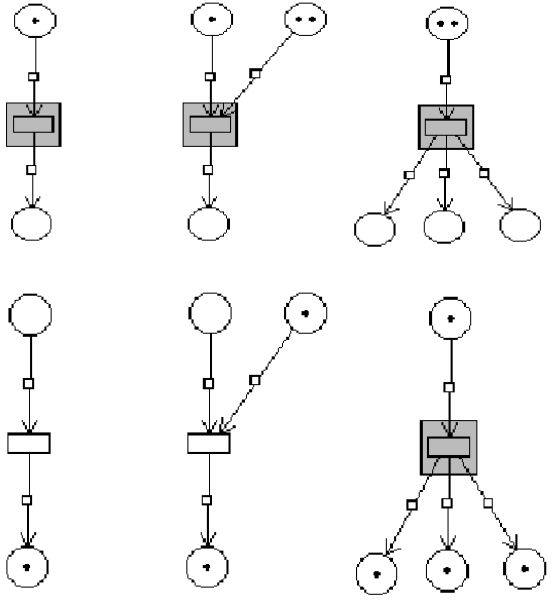
\includegraphics[width=.5\textwidth]{software-engineering/petri-net/petrinet-execution-examples-v2}
	\end{block:ie}
\end{frame}


\begin{frame}
	\frametitle{Rede de Petri}
	\framesubtitle{Funcionamento}
	
	\begin{block:ie}{Mais um exemplo (1/2)}
		\centering
		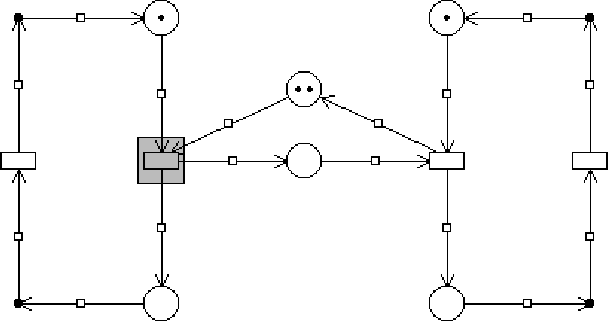
\includegraphics[width=.85\textwidth]{software-engineering/petri-net/petrinet-execution-example1-1}
	\end{block:ie}
\end{frame}

\begin{frame}
	\frametitle{Rede de Petri}
	\framesubtitle{Funcionamento}
	
	\begin{block:ie}{Mais um exemplo (2/2)}
		\centering
		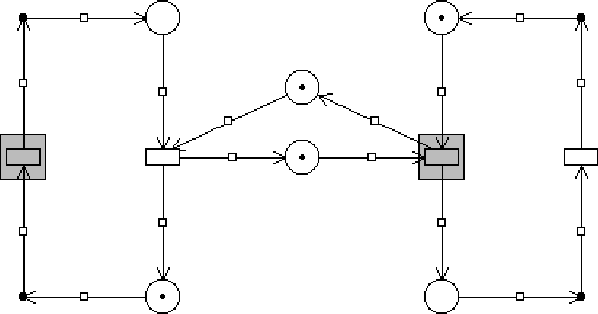
\includegraphics[width=.85\textwidth]{software-engineering/petri-net/petrinet-execution-example1-2}
	\end{block:ie}
\end{frame}


\begin{frame}
	\frametitle{Rede de Petri colorida}
	
	\begin{block:ie}{Exemplo}
		\centering
		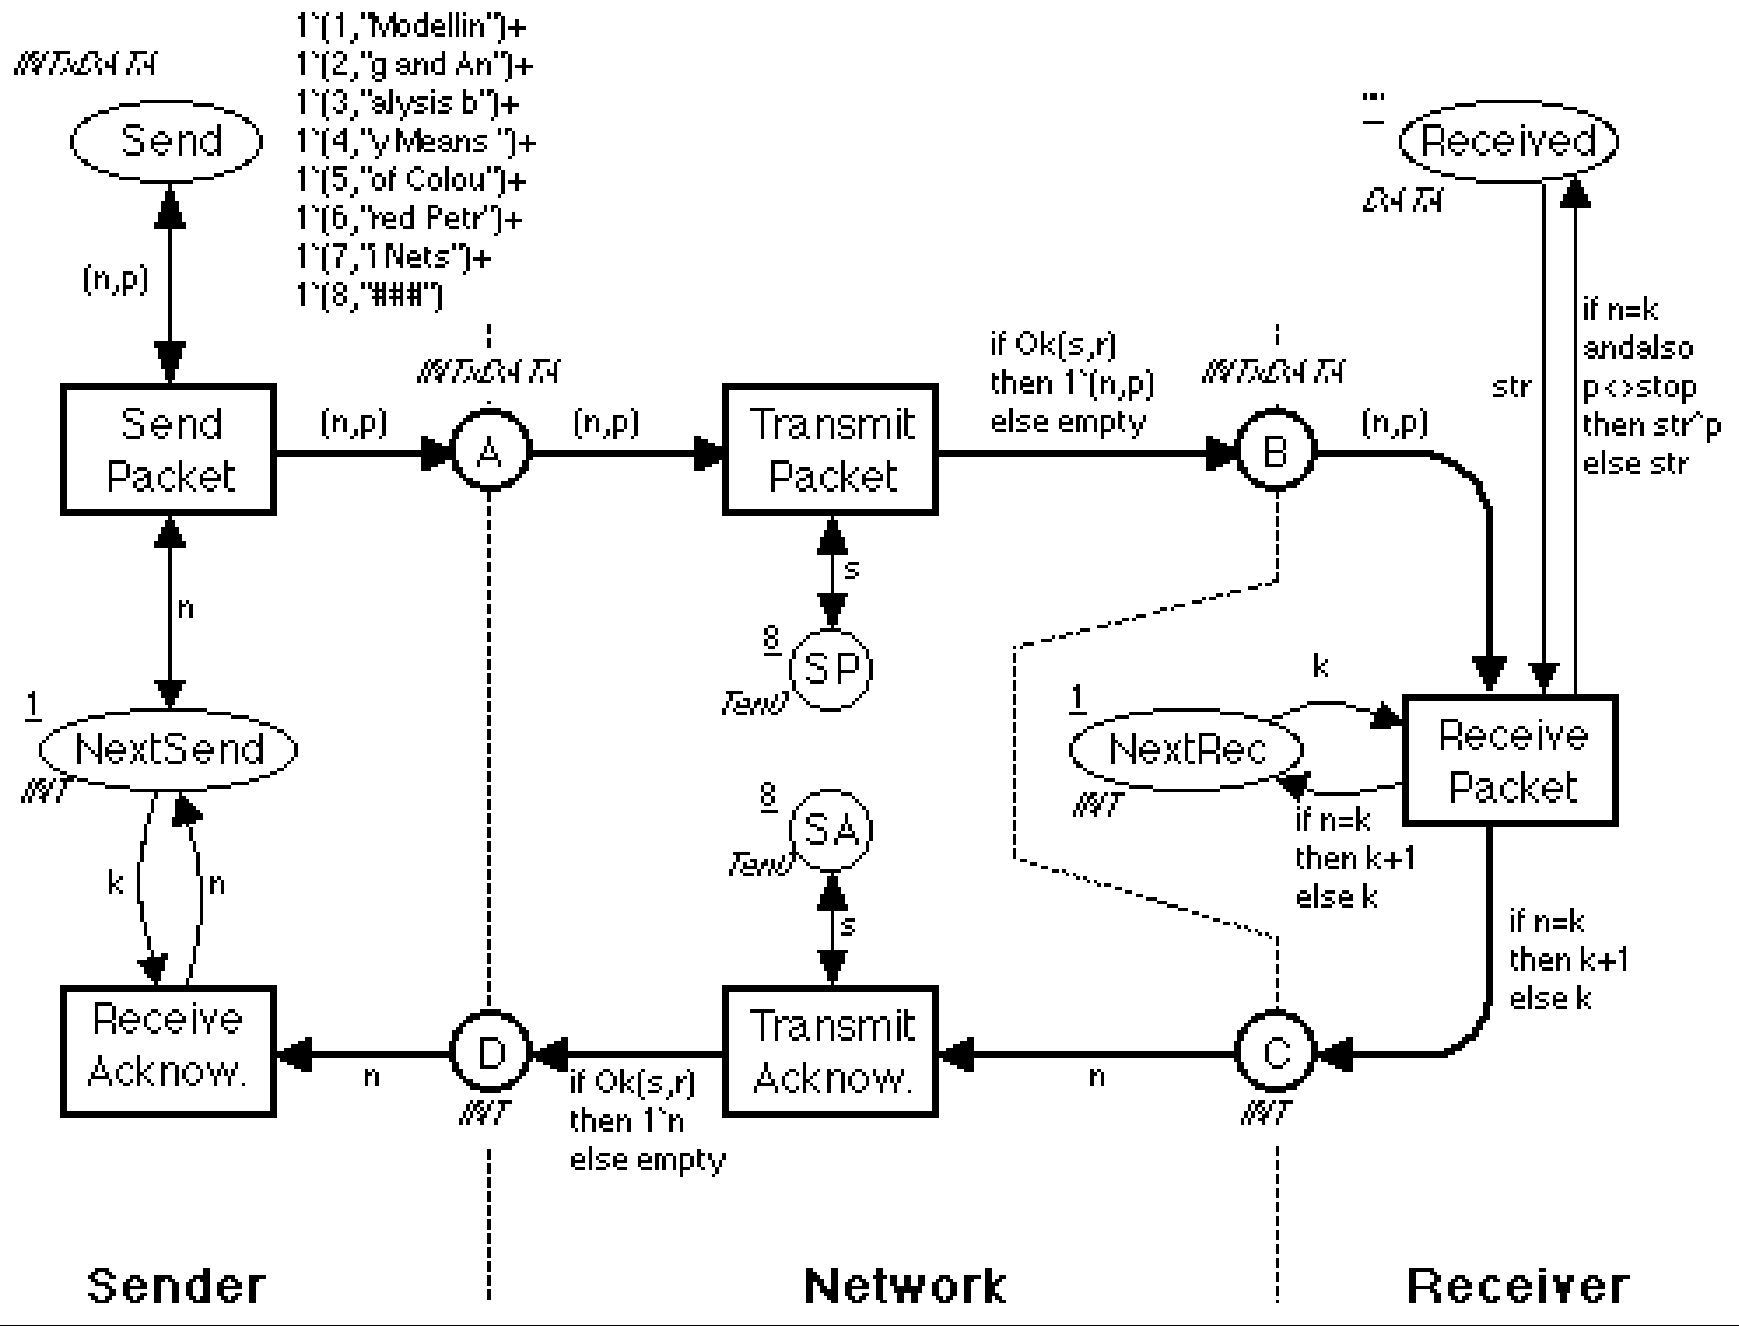
\includegraphics[width=.85\textwidth]{software-engineering/petri-net/cpn-example-network_protocol}
	\end{block:ie}
\end{frame}



\begin{frame}
	\frametitle{Definição de processo}
	\framesubtitle{BPML}
	
	
	
	\begin{block:fact}{Exemplos}
		\begin{itemize}
			\item SEI (Base de conhecimento)
			
			\item \url{https://josegomezdev.medium.com/full-software-development-life-cycle-ca80bb6aae21}
		\end{itemize}
	\end{block:fact}
\end{frame}


\begin{frame}
	\frametitle{Definição de processo}
	\framesubtitle{SPEM}
	
	
	
	\begin{block:fact}{Scrum}
		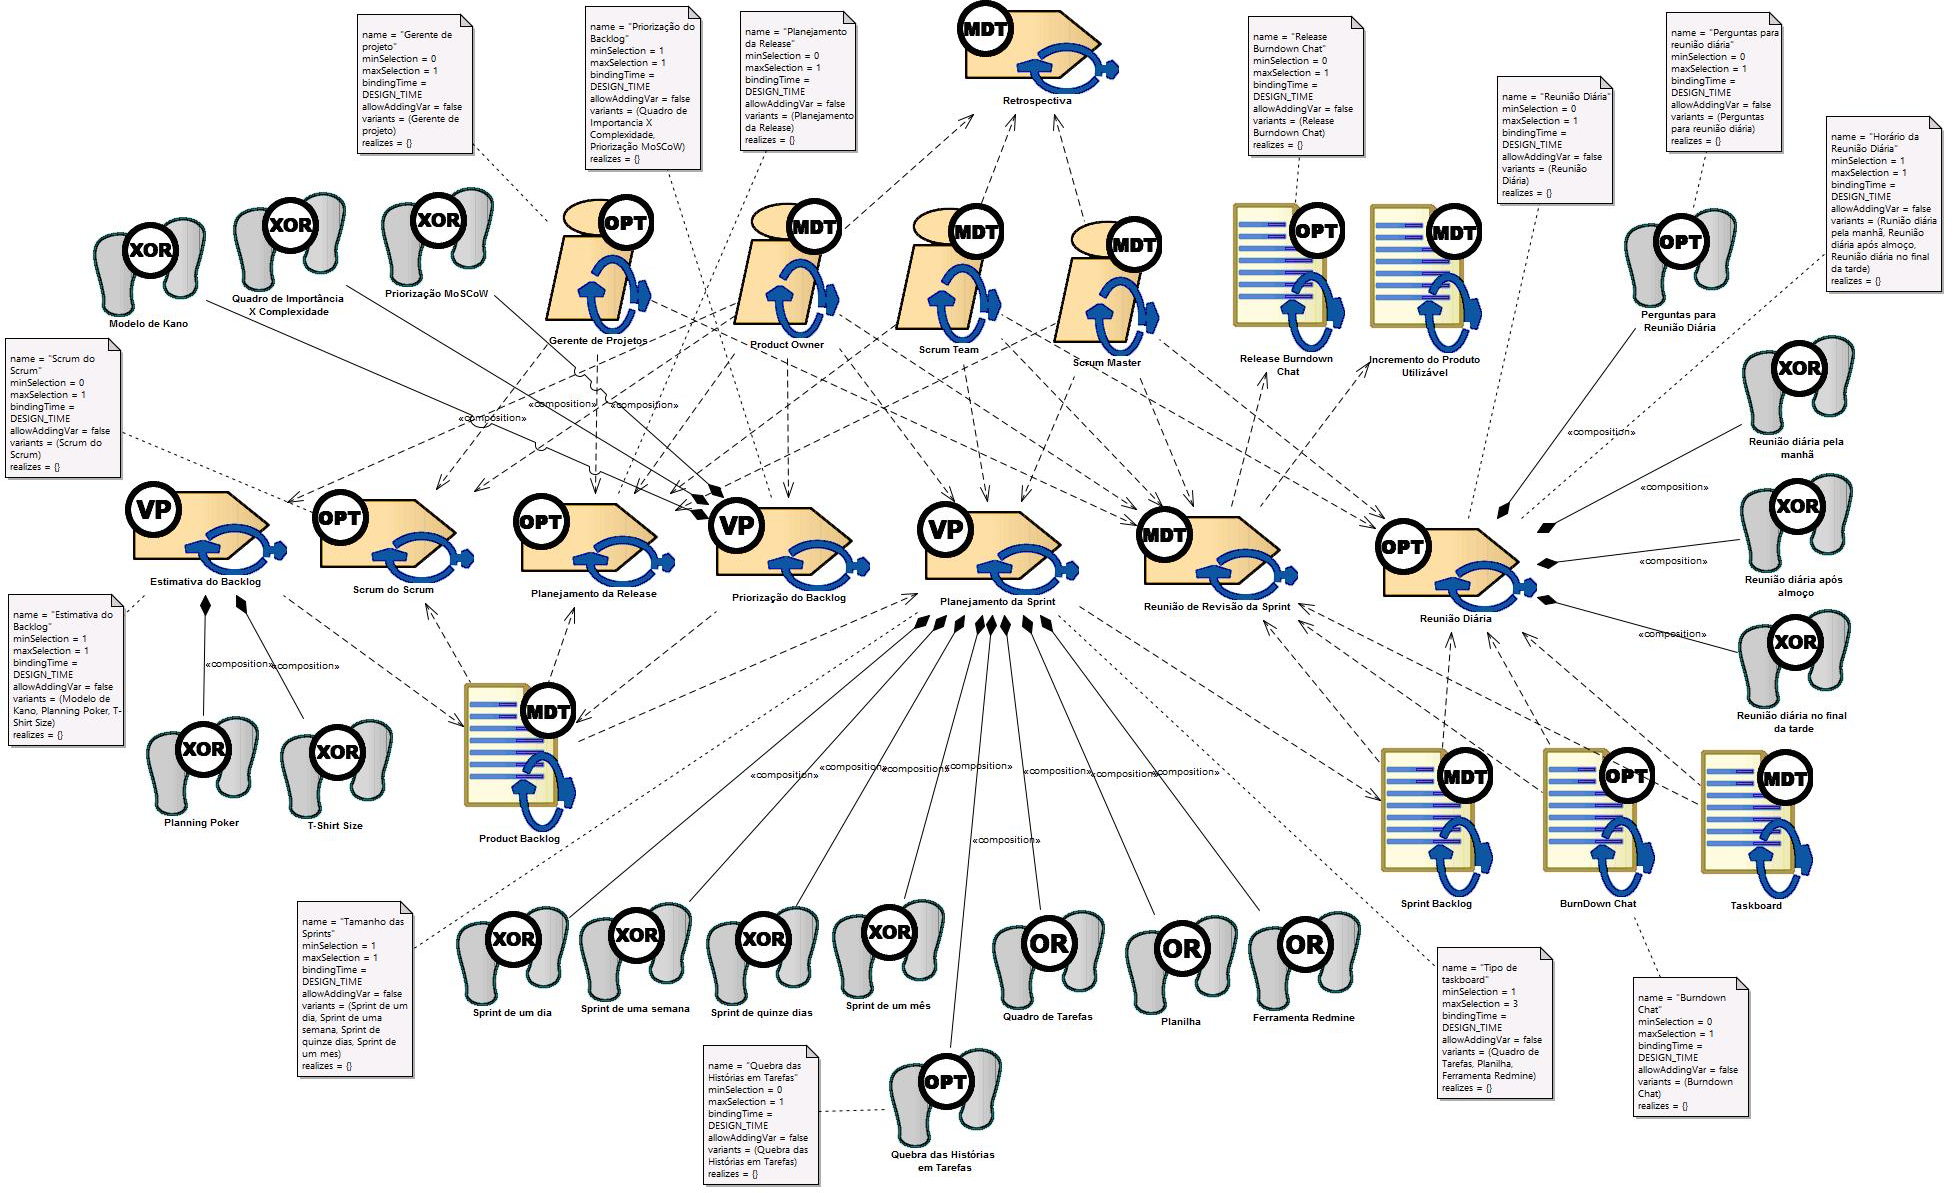
\includegraphics[width=\textwidth]{scrumsprl}
	\end{block:fact}
\end{frame}



\begin{frame}
	\frametitle{Definição de processo}
	\framesubtitle{EPF}
	
	
	\begin{block:concept}{Definição}
		Abordagem composicional que permite a edição, configuração e publicação de processos
		de software.
	\end{block:concept}
	
	\begin{block:fact}{Componentes}
		\begin{itemize}
			\item Method Content: padroniza a representação e gerencia bibliotecas de componentes
			reutilizáveis. Possui a definição de papeis, tarefas, produtos de trabalho e seus
			relacionamentos;
			
			\item Process: determina a sequência das fases, iterações e atividades, e define
			quando realizar as tarefas;
			
			\item Plug-ins: representam um conjunto de Method Content e Process, permitindo a
			customização de um processo;
			
			\item Configurations: seleção de um subconjunto de Method Content para ser
			publicado, visando atender as necessidades de um determinado projeto.
		\end{itemize}
	\end{block:fact}
\end{frame}


\begin{frame}
	\frametitle{Definição de processo}
	\framesubtitle{EPF}
	
	\begin{block:fact}{Exemplos}
		\begin{itemize}
			\item OpenUP: \url{https://magsilva.pro.br/teaching/epf-processes/OpenUP/index.htm}
			\item XP: \url{https://magsilva.pro.br/teaching/epf-processes/XP/index.htm}
			\item Scrum: \url{https://magsilva.pro.br/teaching/epf-processes/Scrum/index.htm}
		\end{itemize}
	\end{block:fact}
\end{frame}


\begin{frame}
	\frametitle{Definição de processo}
	\framesubtitle{EPF}
	
	\begin{block:concept}{Mecanismos para evolução do processo}
		O EPF permite representar variabilidade de artefatos para o controle da evolução e reuso de processos:

		\begin{itemize}
			\item Contribui - adiciona um novo elemento ao elemento base;

			\item Substitui - substitui o elemento base por um novo elemento;

			\item Estende - estende um elemento com as características de um elemento base;

			\item Estende e Substitui - substitui somente os atributos que foram modificados em um novo elemento.
		\end{itemize}
	\end{block:concept}
\end{frame}

%\begin{frame}
%	\frametitle{Definição de processo}
%	\framesubtitle{Linhas de processo de software}
%	
%	\begin{block:concept}{Definição}
%		Estabelece técnicas e mecanismos para a modelagem de similaridades e variabilidades
%		existentes em uma família de processos de software, e a derivação de processos de
%		software customizados que atendam às necessidades específicas de um determinado
%		projeto de desenvolvimento de software.
%	\end{block:concept}
%\end{frame}
%
%
%\begin{frame}[hasnext=false, hasprev=true]
%	\frametitle{Definição de processo}
%	\framesubtitle{Linhas de processo de software}
%	
%	\begin{block:fact}{Exemplo: Scrum}
%		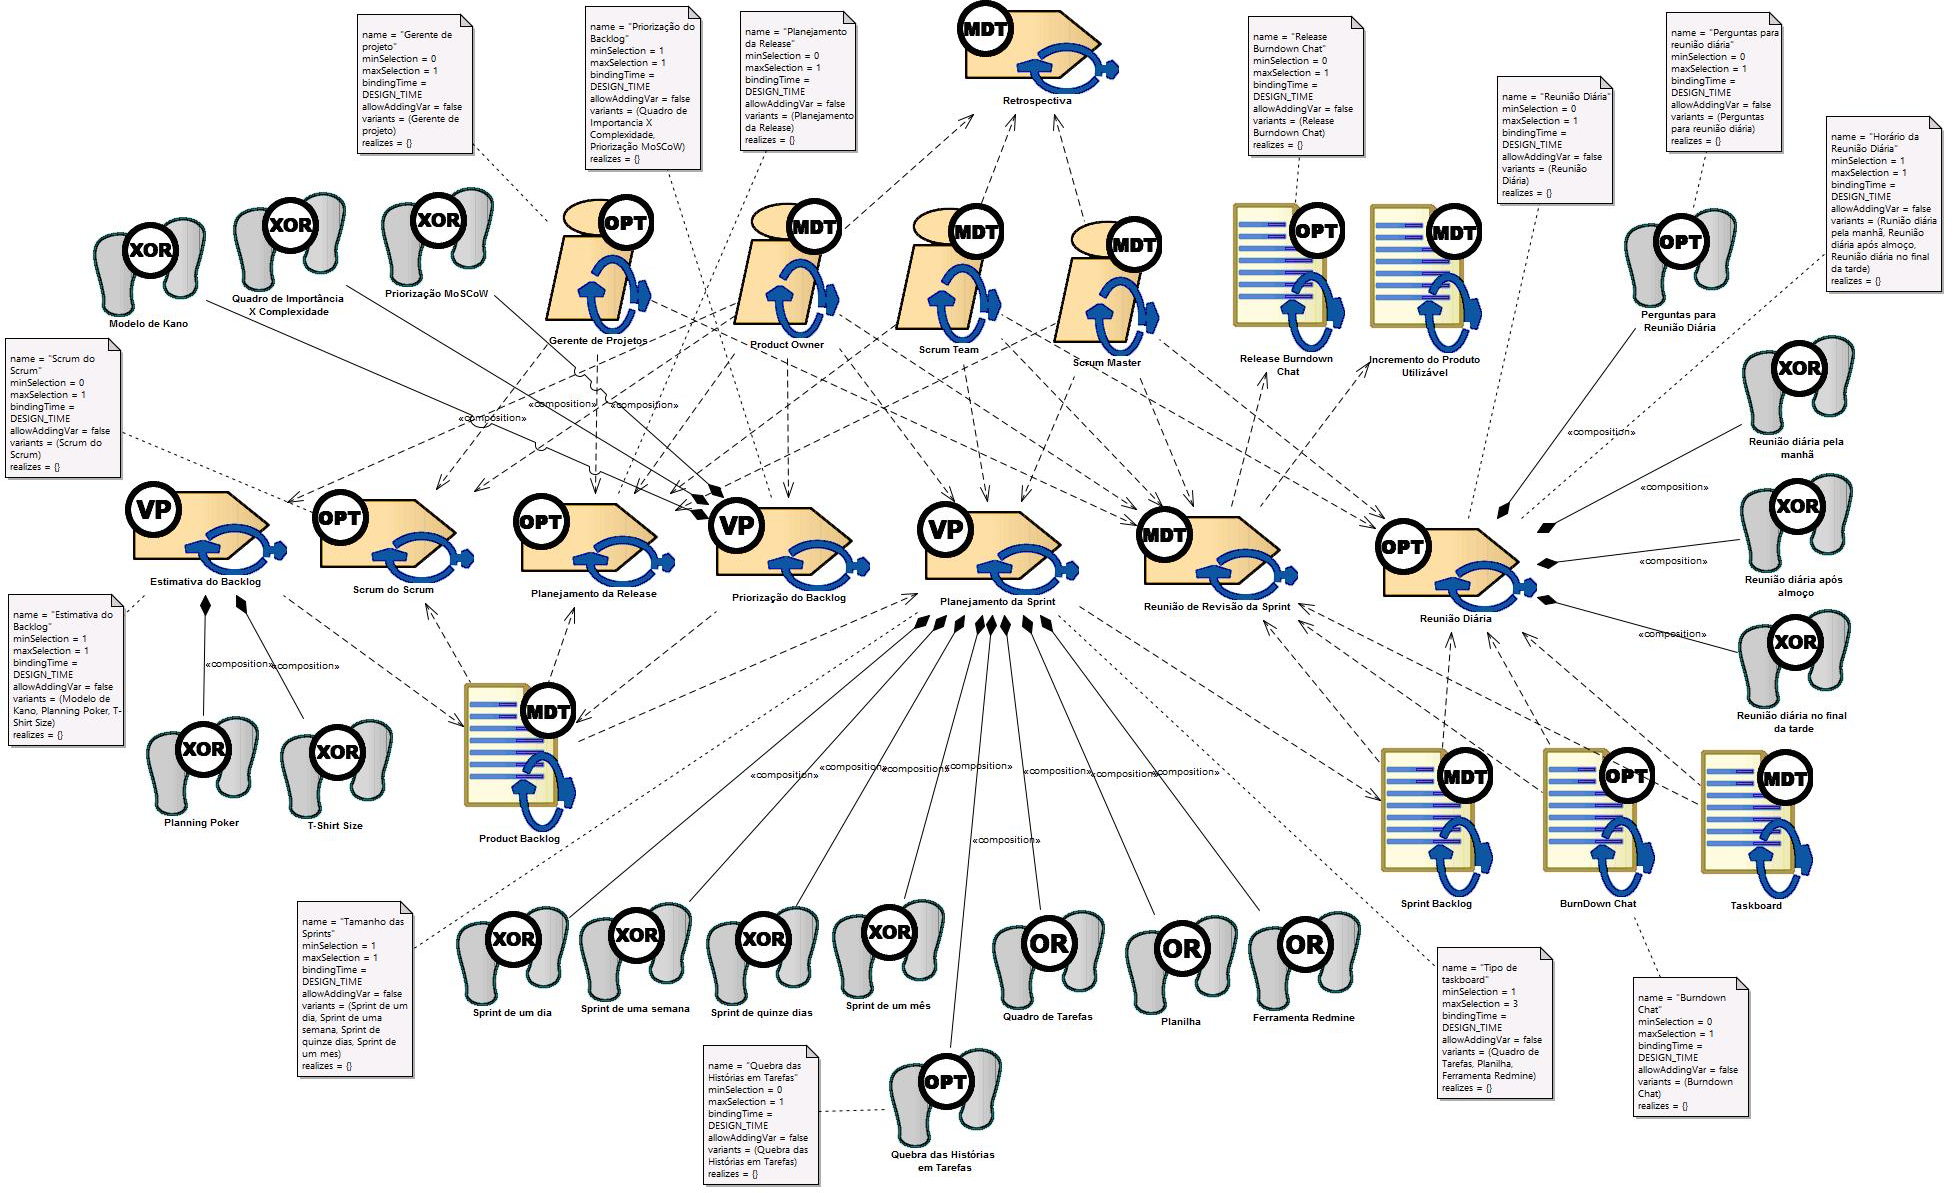
\includegraphics[width=\textwidth]{scrumsprl}
%	\end{block:fact}
%	
%	\note{Linha de Produto para o Scrum, definida com a abordagem composicional SMartySPEM pelo
%	Jaime Dias e Edson Oliveira Jr., da UEM.}
%\end{frame}





\subsection{Qualidade de processo}
\begin{frame}[parent={ie:agenda}, hasnext=true, hasprev=false]
	\frametitle{Qualidade de processo}
	
	\begin{block:concept}{Melhoria de Processo}
		Definição, implantação, medição, gerência, mudança e melhoria do
		processo de engenharia de software.
	\end{block:concept}
	
	\begin{block:fact}{Objetivos}
		\begin{itemize}
			\item Melhorar produtividade
			\begin{itemize}
				\item Diminuir retrabalho/Aumentar reúso
			\end{itemize}
			
			\item Previsibilidade
			\begin{itemize}
				\item Melhorar estimativas
				\item Padronizar qualidade do produto obtido
			\end{itemize}
			
			\item Controlar riscos
			
			\item Aumentar a qualidade do produto
		\end{itemize}
	\end{block:fact}
\end{frame}


\begin{frame}[hasnext=true, hasprev=true]
	\frametitle{Qualidade de processo}
	
	\begin{block:procedure}{Passos}
		\begin{itemize}
			\item Estabelecer infraestrutura para o processo.
			\item Planejar a implantação e alteração do processo.
			\item Implantar e alterar o processo.
			\item Avaliar o processo.
		\end{itemize}
	\end{block:procedure}

	\note{
		\begin{itemize}
			\item Infraestrutura:
			\begin{itemize}
				\item Recursos humanos, atribuição de responsabilidades
				\item Recursos financeiros
				\item Ferramentas
			\end{itemize}
			
			\item Geralmente é necessário ter um grupo de trabalho específico para
			tratar desta infraestrutura:
			\begin{itemize}
				\item Fábrica de experiências
			\end{itemize}
			
			\item Ao invés de começar com a definição de um novo processo, analise
			o processo atual!
			\begin{itemize}
				\item Mapeie as boas práticas
				\item Acrescente novas quando necessário
			\end{itemize}
		\end{itemize}
	}
\end{frame}

% \subsubsection{ISO 15504}
% \begin{frame}[parent={ie:agenda}, hasnext=true, hasprev=false]
	\frametitle{ISO 15504}

	
	\begin{block:concept}{ISO 15504}
	\end{block:concept}
	
	\begin{block:fact}{Exemplos}
		\begin{itemize}
			\item Capacidade determinada pela avaliação dos processos executados pela
			empresa
		\end{itemize}
	\end{block:fact}
\end{frame}


\begin{frame}[hasnext=true, hasprev=true]
	\frametitle{ISO 15504}

	\begin{block:fact}{Níveis}
		\centering
		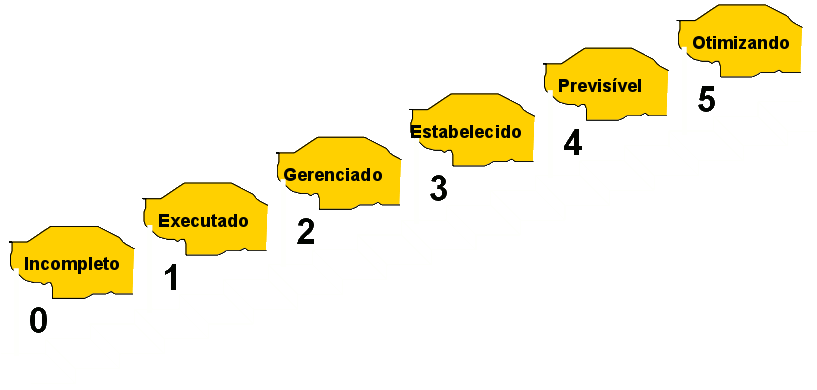
\includegraphics[width=\textwidth]{software-engineering/project-management/process/process-quality/iso15504/iso15504-steps}
	\end{block:fact}
\end{frame}

\begin{frame}
	\frametitle{ISO 15504}

	\begin{block:fact}{}
		Capacidade determinada pela avaliação dos processos executados pela empresa
	\end{block:fact}
	
	\begin{block:fact}{Atributos de processos (e níveis)}
		\begin{itemize}
			\item desempenho do processo (1)
			\item gerência do desempenho do processo (2)
			\item gerência do produtos de trabalho (2)
			\item definição de processo (3)
			\item instanciação de processo (3)
			\item medição de processo (4)
			\item controle de processo (4)
			\item inovação de processo (5)
			\item otimização de processo (5)
		\end{itemize}
	\end{block:fact}
\end{frame}

\begin{frame}[hasnext=false, hasprev=true]
	\frametitle{ISO 15504}

	\begin{block:fact}{Níveis}
		\centering
		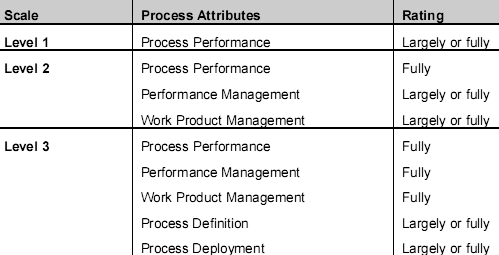
\includegraphics[width=\textwidth]{software-engineering/project-management/process/process-quality/iso15504/iso15504-rating-example}
	\end{block:fact}
\end{frame}



\subsubsection{CMMi}
\begin{frame}[parent={ie:agenda}, hasnext=true, hasprev=false]
	\frametitle{CMMi}

	
	\begin{block:concept}{CMMi}
		Modelo de capacitação de processos de software
	\end{block:concept}
	
	\begin{block:fact}{Organização}
		\begin{itemize}
			\item Organizado em áreas de processo.
			
			\item Cada área de processo define:
			\begin{itemize}
				\item atividades relacionadas,
				\item requisitos para obtenção de um nível no CMMi (metas a serem atendidas)
			\end{itemize}
		\end{itemize}
	\end{block:fact}
	
	\note{Áreas de processo =  antigas KPA - \foreign{Key Process Area}}
\end{frame}


\begin{frame}[hasnext=true, hasprev=true]
	\frametitle{CMMi}

	\begin{block:fact}{CMMi staged}
		\centering
		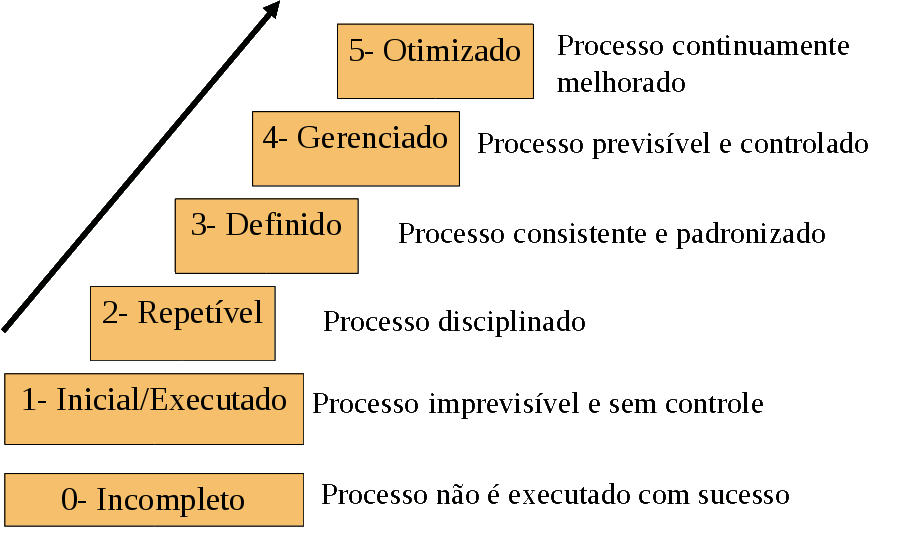
\includegraphics[width=\textwidth]{software-engineering/project-management/process/process-quality/cmmi/cmmi-staged}
	\end{block:fact}
\end{frame}


\begin{frame}
	\frametitle{CMMi}
	\framesubtitle{CMMi staged - Nível 1}
	
	\begin{block:fact}{Nível 1}
		Sucesso é resultado de esforços individuais e heroicos (ou pura sorte)
	\end{block:fact}
	
	\begin{block:fact}{}
		\centering
		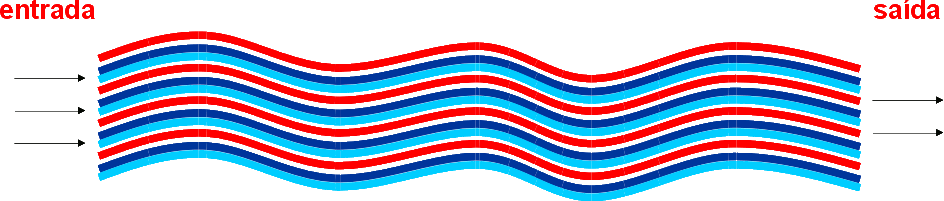
\includegraphics[width=\textwidth]{software-engineering/project-management/process/process-quality/cmmi/cmmi-staged-1}
	\end{block:fact}
\end{frame}


\begin{frame}
	\frametitle{CMMi}
	\framesubtitle{CMMi staged - Nível 1}
	
	\begin{block:fact}{Nível 1}
		Sucesso é resultado de esforços individuais e heroicos (ou pura sorte)
	\end{block:fact}
	
	\begin{block:fact}{Sintomas}
		\begin{itemize}
			\item cronogramas e planos irrealistas
			\item aquilo que é planejado não é seguido (em parte porque eles não tem credibilidade)
			\item cliente só avalia os requisitos no momento da 	entrega
			\item processo de desenvolvimento pula dos requisitos para implementação (para que projeto!)
			\item documentação inexistente
			\item reações contrárias à atividades de melhoria de qualidade
		\end{itemize}
	\end{block:fact}
\end{frame}


\begin{frame}
	\frametitle{CMMi}
	\framesubtitle{CMMi staged - Nível 2}
	
	\begin{block:fact}{Nível 2 -- Repetível}
		\begin{itemize}
		 \item Processo básico de gerência, com controle de custos, prazos e escopo.
		 \item Empresa consegue repetir o sucesso de projetos anteriores em aplicações
		 similares.
		\end{itemize}
	\end{block:fact}
	
	\begin{block:fact}{}
		\centering
		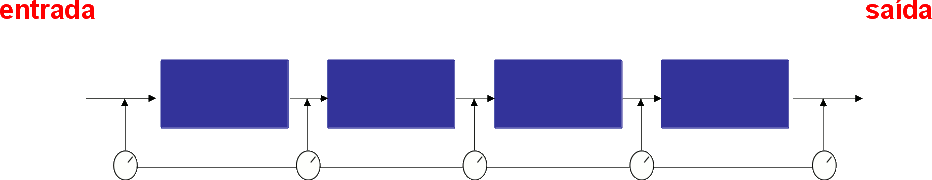
\includegraphics[width=\textwidth]{software-engineering/project-management/process/process-quality/cmmi/cmmi-staged-2}
	\end{block:fact}
\end{frame}


\begin{frame}
	\frametitle{CMMi}
	\framesubtitle{CMMi staged - Nível 2}
	
	\begin{block:fact}{Nível 2 -- Repetível}
		\begin{itemize}
			\item Processo básico de gerência, com controle de custos, prazos e escopo.
			\item Empresa consegue repetir o sucesso de projetos anteriores em aplicações
			similares.
		\end{itemize}
	\end{block:fact}
	
	\begin{block:fact}{Áreas de processo}
		\begin{itemize}
			\small
			\item Gerência de requisitos.
			\item Planejamento de projetos; Monitoramento e controle de projetos.
			\item Garantia de qualidade de processo e de software.
			\item Gerência de contratos com fornecedores.
			\item Gerência de configuração.
			\item Medição e análise.
		\end{itemize}
	\end{block:fact}
\end{frame}

\begin{frame}
	\frametitle{CMMi}
	\framesubtitle{CMMi staged - Nível 2}
	
	\begin{block:fact}{Nível 2 -- Repetível}
		\begin{itemize}
			\item Processo básico de gerência, com controle de custos, prazos e escopo.
			\item Empresa consegue repetir o sucesso de projetos anteriores em aplicações
			similares.
		\end{itemize}
	\end{block:fact}
	
	\begin{block:fact}{Evidências de organizações nível 2:}
		\begin{itemize}
			\item Empresa consegue cumprir compromissos de requisitos, prazos e custos.
			\\No entanto, gerente de projeto não consegue alterar o plano em frente a problemas
			graves.
			\item Evolução controlada dos artefatos de software.
			\item Ainda apresenta resistência às atividades de melhoria de qualidade.
		\end{itemize}
	\end{block:fact}
\end{frame}

\begin{frame}
	\frametitle{CMMi}
	\framesubtitle{CMMi staged - Nível 3}
	
	\begin{block:fact}{Nível 3 -- Definido}
		\begin{itemize}
			\item Processo de software padronizado
			\begin{itemize}
				\item Existe um modelo de processo (processo-padrão) e cada projeto
				utiliza uma versão especializada desse processo
			\end{itemize}
			\item Em cada etapa do desenvolvimento, a organização interna das tarefas
			está definida e visível
		\end{itemize}
	\end{block:fact}
	
	\begin{block:fact}{}
		\centering
		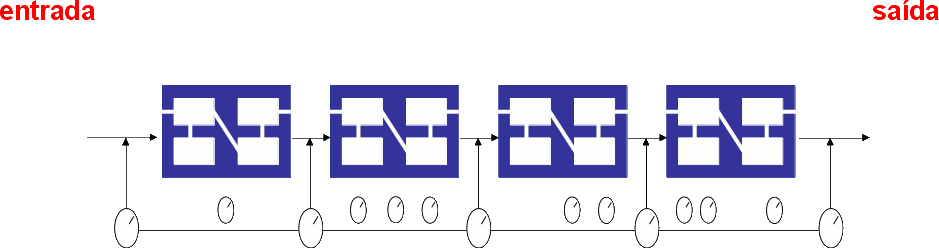
\includegraphics[width=\textwidth]{software-engineering/project-management/process/process-quality/cmmi/cmmi-staged-3}
	\end{block:fact}
\end{frame}

\begin{frame}
	\frametitle{CMMi}
	\framesubtitle{CMMi staged - Nível 3}
	
	\begin{block:fact}{Nível 3 -- Definido}
		\begin{itemize}
			\item Processo de software padronizado
			\begin{itemize}
				\item Existe um modelo de processo (processo-padrão) e cada projeto
				utiliza uma versão especializada desse processo
			\end{itemize}
			\item Em cada etapa do desenvolvimento, a organização interna das tarefas
			está definida e visível
		\end{itemize}
	\end{block:fact}
	
	\begin{block:fact}{Áreas de processo}
		\begin{itemize}
			\small
			\item Gerência de projeto integrada
			\item Definição do processo organizacional
			\item Foco no processo organizacional; Treinamento organizacional
			\item Desenvolvimento de requisitos; Integração do produto
			\item Verificação;  Validação
			\item Gerência de riscos; Análise de decisão e resolução
		\end{itemize}
	\end{block:fact}
\end{frame}

\begin{frame}
	\frametitle{CMMi}
	\framesubtitle{CMMi staged - Nível 3}
	
	\begin{block:fact}{Nível 3 -- Definido}
		\begin{itemize}
			\item Processo de software padronizado
			\begin{itemize}
				\item Existe um modelo de processo (processo-padrão) e cada projeto
				utiliza uma versão especializada desse processo
			\end{itemize}
			\item Em cada etapa do desenvolvimento, a organização interna das tarefas
			está definida e visível
		\end{itemize}
	\end{block:fact}
	
	\begin{block:fact}{Evidências de organizações nível 3}
		\begin{itemize}
			\item Processo padronizado e adaptado para cada projeto.
			\item Abandono de um desenvolvedor não causa prejuízo irreparável ao projeto.
			\item Aplicação de técnicas para melhoria de processo é viável.
		\end{itemize}
	\end{block:fact}
\end{frame}

\begin{frame}
	\frametitle{CMMi}
	\framesubtitle{CMMi staged - Nível 4}
	
	\begin{block:fact}{Nível 4 -- Gerenciado}
		\begin{itemize}
			\item Processo de software padronizado e controlado
			\item Métricas coletadas e utilizadas para gerenciar o projeto
		\end{itemize}
	\end{block:fact}
	
	\begin{block:fact}{}
		\centering
		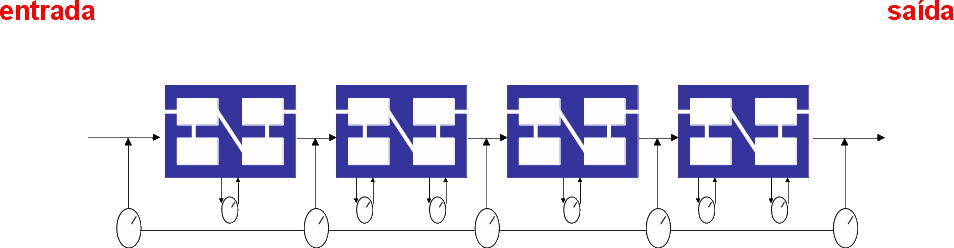
\includegraphics[width=\textwidth]{software-engineering/project-management/process/process-quality/cmmi/cmmi-staged-4}
	\end{block:fact}
\end{frame}


\begin{frame}
	\frametitle{CMMi}
	\framesubtitle{CMMi staged - Nível 4}
	
	\begin{block:fact}{Nível 4 -- Gerenciado}
		\begin{itemize}
			\item Processo de software padronizado e controlado
			\item Métricas coletadas e utilizadas para gerenciar o projeto
		\end{itemize}
	\end{block:fact}
	
	\begin{block:fact}{Áreas de processo}
		\begin{itemize}
			\item Gerência quantitativa dos processos
			\item Desempenho do processo organizacional
		\end{itemize}
	\end{block:fact}
		

	\begin{block:fact}{Evidências de organizações nível 4}
		\begin{itemize}
			\item Organização estabelece metas (quantitativas) para as atividades do
			processo e produtos produzidos
			\item Medidas são coletadas para todos os projetos e para suas atividades
			\item Desvios de execução das atividades são prontamente detectados
		\end{itemize}
	\end{block:fact}
\end{frame}



\begin{frame}
	\frametitle{CMMi}
	\framesubtitle{CMMi staged - Nível 5}
	
	\begin{block:fact}{Nível 5 -- Otimizado}
		\begin{itemize}
			\item Melhoria contínua do processo
			\item Implantação planejada e controlada de melhorias
		\end{itemize}
	\end{block:fact}
	
	\begin{block:fact}{}
		\centering
		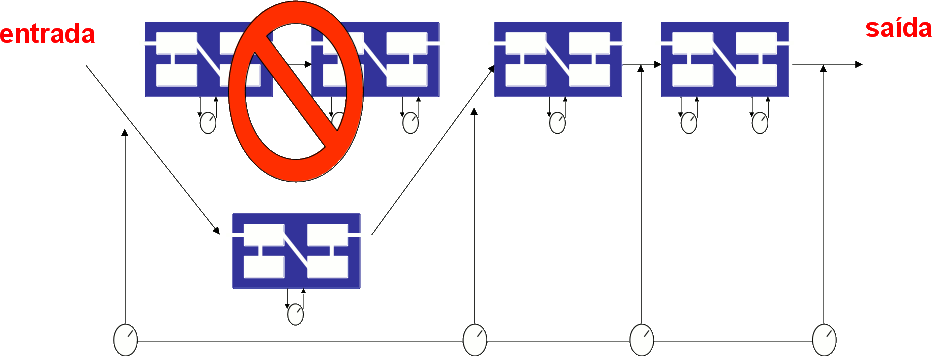
\includegraphics[width=\textwidth]{software-engineering/project-management/process/process-quality/cmmi/cmmi-staged-5}
	\end{block:fact}
\end{frame}


\begin{frame}
	\frametitle{CMMi}
	\framesubtitle{CMMi staged - Nível 5}
	
	\begin{block:fact}{Nível 5 -- Otimizado}
		\begin{itemize}
			\item Melhoria contínua do processo
			\item Implantação planejada e controlada de melhorias
		\end{itemize}
	\end{block:fact}
	
	\begin{block:fact}{Áreas de processo}
		\begin{itemize}
			\item Análise de causas e resolução
			\item Inovação e implantação na organização
		\end{itemize}
	\end{block:fact}


	\begin{block:fact}{Evidências de organizações nível 5}
		\begin{itemize}
			\item Organização engajada em melhoria contínua do processo
			\item Efeitos de cada técnica aplicada são mensuráveis
			\item Para cada melhoria, é possível estabelecer o custo e o benefício
		\end{itemize}
	\end{block:fact}
\end{frame}

\begin{frame}
	\frametitle{CMMi}
	\framesubtitle{Áreas de processo}
	
	\begin{block:fact}{}
		\centering
		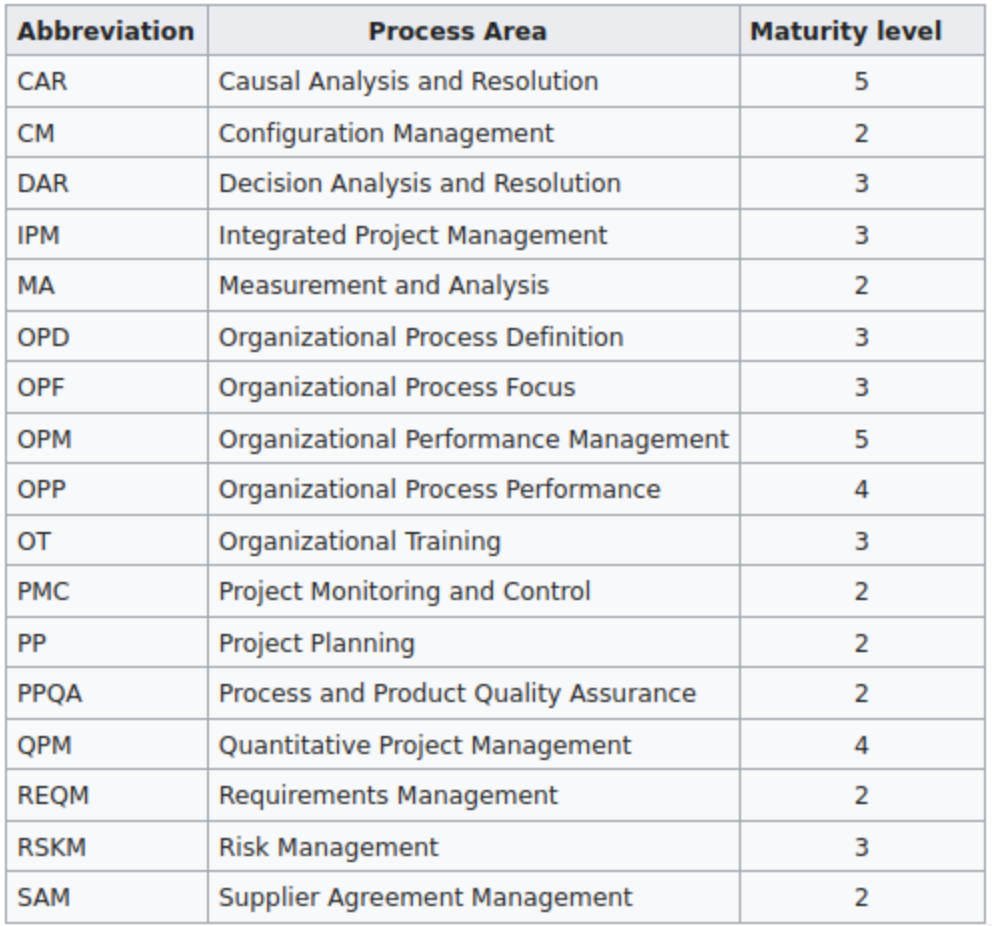
\includegraphics[width=.8\textwidth]{software-engineering/project-management/process/process-quality/cmmi/cmmi-pa}

	\end{block:fact}
\end{frame}


\begin{frame}
	\frametitle{CMMi}
	\framesubtitle{CMMi contínuo}
	
	\begin{block:fact}{Diferença entre contínuo e staged}
		Ao invés de medir a maturidade, é medida a capacidade de uma ou mais áreas
		de processo.
	\end{block:fact}
	
	\begin{block:fact}{}
		\centering
		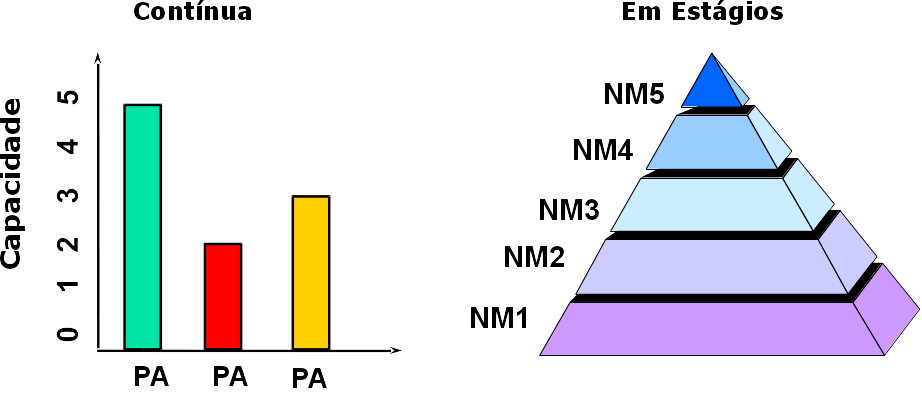
\includegraphics[width=\textwidth]{software-engineering/project-management/process/process-quality/cmmi/cmmi-continuous}
	\end{block:fact}
\end{frame}



\begin{frame}
	\frametitle{CMMi}
	\framesubtitle{Empresas com CMMi}
	
	\begin{block:fact}{}
		\url{https://cmmiinstitute.com/pars}
	\end{block:fact}
	
	\begin{block:fact}{Nível 5 (staged)}
		\begin{itemize}
			\item Critical Software, S.A.
			\item everis
			\item HP Enterprise Services
			\item IBM
			\item Spread Sistemas e Automação Ltda
			\item Synapsis Brasil S.A.
			\item Tata Consultancy Services Limited
		\end{itemize}
	\end{block:fact}

		\begin{block:fact}{Nível 4 (staged)}
		\begin{itemize}
			\item CPM Braxis S.A. (Capgemini)
		\end{itemize}
	\end{block:fact}
\end{frame}



\subsubsection{MPS.BR}
\begin{frame}[parent={ie:agenda}, hasnext=true, hasprev=false]
	\frametitle{MPS.BR}
	
	\begin{block:concept}{Objetivo}
		Melhoria de processos de software nas micros, pequenas e médias empresas
		(PMEs), a um custo acessível, em diversos locais do país.
	\end{block:concept}
	
	\begin{block:fact}{}
		\begin{itemize}
			\item CMMi + ISO 15504 + ISO 12207
			\item Softex + Governo + universidades
		\end{itemize}
	\end{block:fact}
\end{frame}


\begin{frame}[hasnext=true, hasprev=true]
	\frametitle{MPS.BR}
	
	\begin{block:fact}{Base técnica}
		\centering
		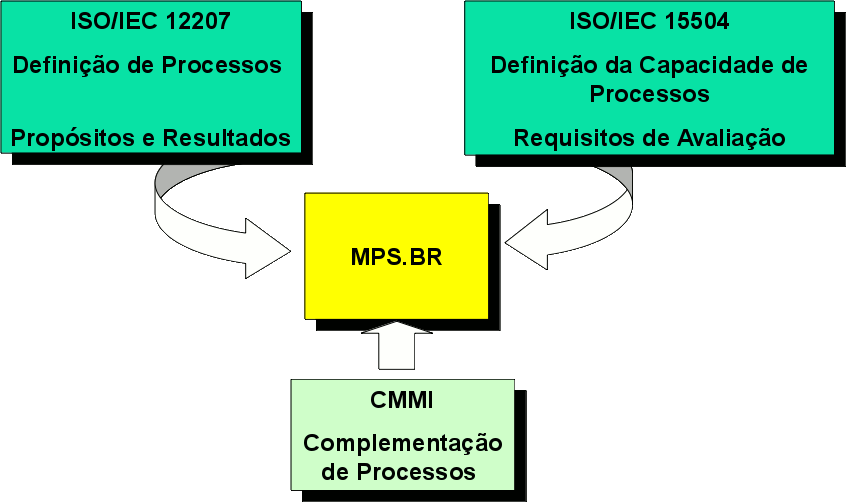
\includegraphics[width=\textwidth]{software-engineering/project-management/process/process-quality/mpsbr/technical-base}
	\end{block:fact}
\end{frame}


\begin{frame}
	\frametitle{MPS.BR}
	
	\begin{block:fact}{Estrutura}
		\centering
		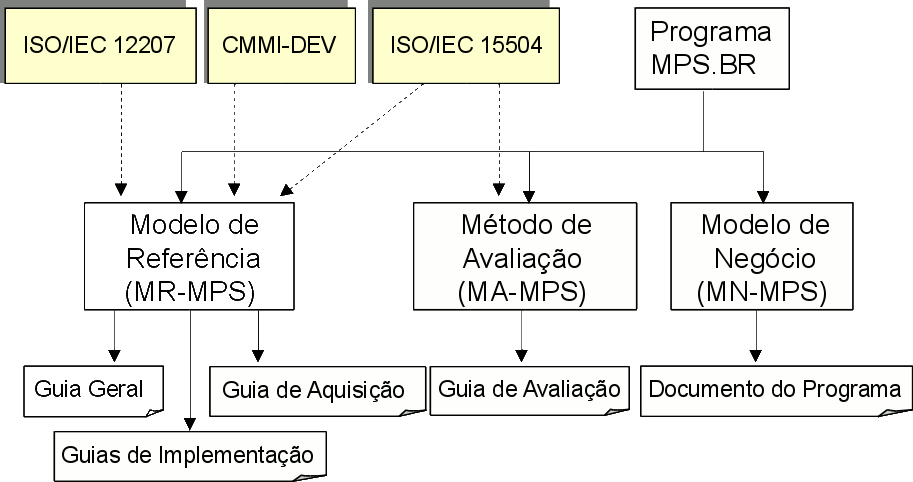
\includegraphics[width=\textwidth]{software-engineering/project-management/process/process-quality/mpsbr/structure}
	\end{block:fact}
\end{frame}



\begin{frame}
	\frametitle{MPS.BR}
	\framesubtitle{Guia geral}
	
	\begin{block:concept}{Guia geral}
		Descreve o Modelo de Referência para Melhoria de Processo de Software
		(MR-MPS)
	\end{block:concept}

	\begin{block:fact}{Características}
		\begin{itemize}
			\item Níveis de maturidade
			
			\item Processos
			\begin{itemize}
				\item Propósitos
				\item Resultados esperados
			\end{itemize}
			
			\item Atributos de processo
			\begin{itemize}
				\item Resultados esperados
			\end{itemize}
		\end{itemize}
	\end{block:fact}
	
	\note{
		As atividades e tarefas necessárias para atender aos propósitos e obter os
		resultados esperados de um processo não são definidos!
	}
\end{frame}



\begin{frame}
	\frametitle{MPS.BR}
	\framesubtitle{Níveis de maturidade}
	
	\begin{block:fact}{Níveis de maturidade}
		\centering
		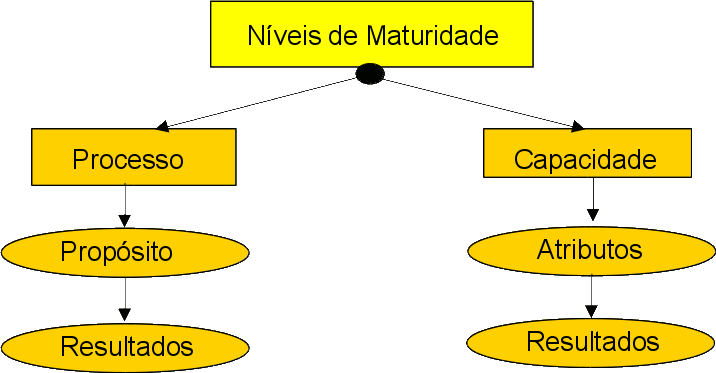
\includegraphics[width=\textwidth]{software-engineering/project-management/process/process-quality/mpsbr/maturity-level}
	\end{block:fact}
\end{frame}



\begin{frame}
	\frametitle{MPS.BR}
	\framesubtitle{Níveis de maturidade}
	
	\begin{block:fact}{Níveis}
		\begin{itemize}
			\item A (em otimização)
			\item B (gerenciado quantitativamente)
			\item C (definido)
			\item D (largamente definido)
			\item E (parcialmente definido)
			\item F (gerenciado)
			\item G (parcialmente gerenciado)
		\end{itemize}
	\end{block:fact}
\end{frame}


\begin{frame}
	\frametitle{MPS.BR}
	\framesubtitle{Níveis de maturidade}
	
	\begin{block:fact}{Níveis de maturidade e processos}
		\centering
		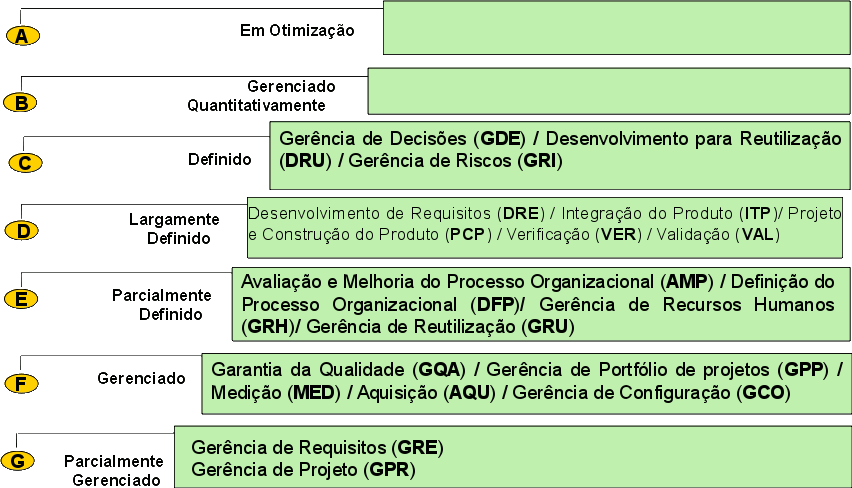
\includegraphics[width=\textwidth]{software-engineering/project-management/process/process-quality/mpsbr/levels-processes}
	\end{block:fact}
\end{frame}


\begin{frame}
	\frametitle{MPS.BR}
	\framesubtitle{Níveis de maturidade}
	
	\begin{block:concept}{Capacidade de processo}
		Expressa o grau de refinamento e institucionalização com que o processo é
		executado na organização ou unidade organizacional, grau este medido pelo
		atendimento de atributos de processo.
	\end{block:concept}

	\begin{block:fact}{Atributos de processo}
		\begin{itemize}
			\item AP 1.1 -- processo é executado
			\item AP 2.1 -- processo é gerenciado
			\item AP 2.2 -- produtos de trabalho do processo são gerenciados
			\item AP 3.1 -- processo é definido
			\item AP 3.2 -- processo está implementado
			\item AP 4.1 -- processo é medido
			\item AP 4.2 -- processo é controlado
			\item AP 5.1 -- processo é objeto de inovações
			\item AP 5.2 -- O processo é otimizado continuamente
		\end{itemize}
	\end{block:fact}
	
	\note{
		\begin{itemize}
			\item Está relacionada com o atendimento aos atributos de processo (AP)
			associados aos processos de cada nível de maturidade.
			\item Cada AP está relacionado com um conjunto de resultados esperados de
			atributo de processo (RAP).
		\end{itemize}
	}
\end{frame}


\begin{frame}
	\frametitle{MPS.BR}
	\framesubtitle{Níveis de maturidade}
	
	\begin{block:fact}{Atributos de processo e resultados esperados}
		Cada AP está relacionado com um conjunto de resultados esperados de atributo de processo (RAP).
	\end{block:fact}
	
	\begin{block:fact}{Exemplo de AP - RAP}
		\begin{itemize}
			\item AP 1.1 -- Processo é executado
			\begin{itemize}
				\item RAP 1. O processo atinge seus resultados definidos
			\end{itemize}
	
			\item AP 2.1 – O processo é gerenciado
			\begin{itemize}
				\item RAP 2. Existe uma política organizacional estabelecida e mantida
				para o processo.
				\item RAP 3. A execução do processo é planejada.
			\end{itemize}
		\end{itemize}
	\end{block:fact}
\end{frame}


\begin{frame}
	\frametitle{MPS.BR}
	\framesubtitle{Níveis de maturidade, processos e capacidades}
	
	\begin{block:fact}{}
		\centering
		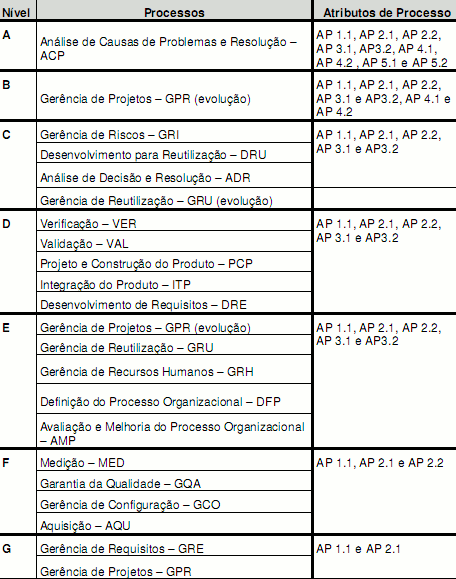
\includegraphics[width=.6\textwidth]{software-engineering/project-management/process/process-quality/mpsbr/levels-processes-capacities}
	\end{block:fact}
\end{frame}


\begin{frame}
	\frametitle{MPS.BR}
	\framesubtitle{Guia geral. Nível G. Gerência de Projetos}
	
	\begin{block:concept}{Propósito}
		Estabelecer e manter planos que e definem atividades, recursos e
		responsabilidades do projeto e que forneçam informações sobre o 
		andamento do projeto que permitam a realização de correções quando houver
		desvios significativos no desempenho. 
	\end{block:concept}

	\begin{block:fact}{Resultados esperados}
		\small
		\begin{itemize}
			\item GPR 1. O escopo do trabalho para o projeto é definido
			\item GPR 2. As tarefas e os produtos do projeto são dimensionados
			utilizando métodos apropriados
			\item GPR 3. O modelo e as fases do ciclo de vida do projeto são
			definidos
			\item GPR 4. (Até o nível F) O esforço e o custo para a execução das
			tarefas e dos produtos de trabalho são estimados com base em dados
			histórios ou referências técnicas
			\item \ldots
		\end{itemize}
	\end{block:fact}
\end{frame}



\begin{frame}
	\frametitle{MPS.BR}
	\framesubtitle{Guia geral. Nível G. Gerência de Projetos}
	
	\begin{block:fact}{Nível G}
		\centering
		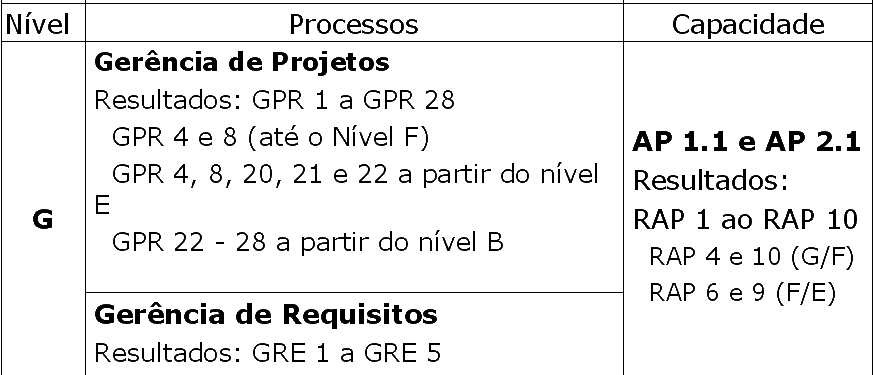
\includegraphics[width=\textwidth]{software-engineering/project-management/process/process-quality/mpsbr/mpsbr-level-g}
	\end{block:fact}
\end{frame}



\begin{frame}
	\frametitle{MPS.BR}
	\framesubtitle{Avaliação}
	
	\begin{block:procedure}{Passos para caracterização de nível}
		\begin{enumerate}
			\item Caracterizar o grau de implementação de cada resultado esperado do
			processo e de cada resultado de atributo de processo \textbf{em cada projeto}
		
			\item Caracterizar inicialmente o grau de implementação de cada resultado
			esperado do processo e de cada resultado de atributo do processo \textbf{na UO}
		
			\item Caracterizar inicialmente o grau de implementação de cada atributo de
			processo \textbf{na UO}

			\item Caracterizar o grau de implementação dos processos \textbf{na UO}

			\item Atribuir nível MPS.BR.
		\end{enumerate}
	\end{block:procedure}
\end{frame}


\begin{frame}
	\frametitle{MPS.BR}
	\framesubtitle{Grau de implementação}
	
	\begin{block:fact}{Caracterização do resultado esperado de processos e
	atributos em cada projeto}
		\centering
		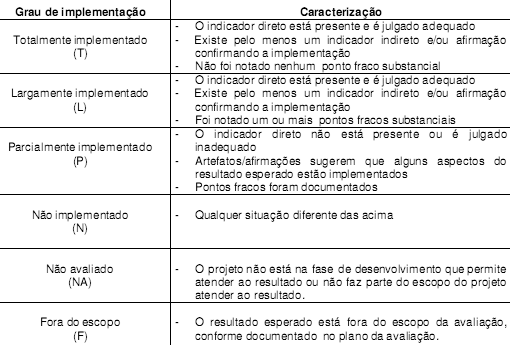
\includegraphics[width=.95\textwidth]{software-engineering/project-management/process/process-quality/mpsbr/mpsbr-implementation-ratings}
	\end{block:fact}
\end{frame}



\begin{frame}
	\frametitle{MPS.BR}
	\framesubtitle{Grau de implementação}
	
	\begin{block:fact}{Caracterização do resultado esperado de processos e
	atributos na UO}
		\centering
		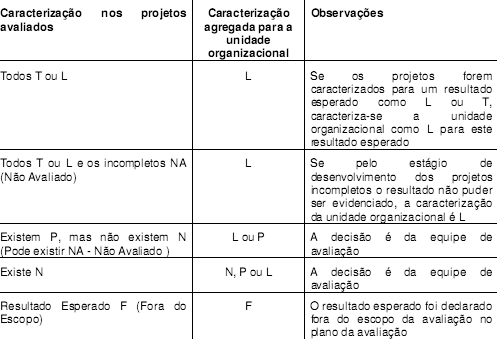
\includegraphics[width=.95\textwidth]{software-engineering/project-management/process/process-quality/mpsbr/mpsbr-implementation-ratings-uo}
	\end{block:fact}
\end{frame}


\begin{frame}
	\frametitle{MPS.BR}
	\framesubtitle{Grau de implementação}
	
	\begin{block:fact}{Caracterização do resultado esperado de atributos na UO}
		\centering
		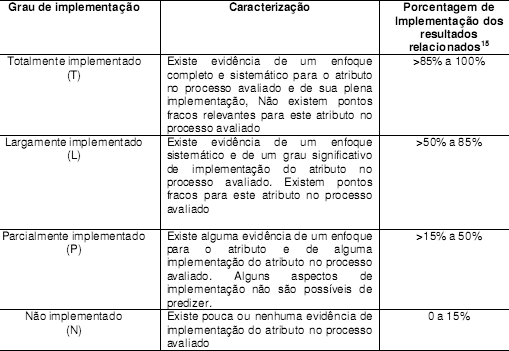
\includegraphics[width=\textwidth]{software-engineering/project-management/process/process-quality/mpsbr/mpsbr-attribute-ratings-uo}
	\end{block:fact}
\end{frame}



\begin{frame}
	\frametitle{MPS.BR}
	\framesubtitle{Grau de implementação}
	
	\begin{block:fact}{Caracterização do nível}
		Um processo está SATISFEITO quando:
		\begin{itemize}
			\item Todos os resultados esperados para o processo foram caracterizados
			como T (Totalmente Implementado) ou L (Largamente Implementado).
			
			\item Tem-se resultados para os atributos do processo, conforme a tabela
			apresentada.
		\end{itemize}
	\end{block:fact}
\end{frame}

\begin{frame}
	\frametitle{MPS.BR}
	\framesubtitle{Grau de implementação}
	
	\begin{block:fact}{Caracterização do nível}
		\centering
		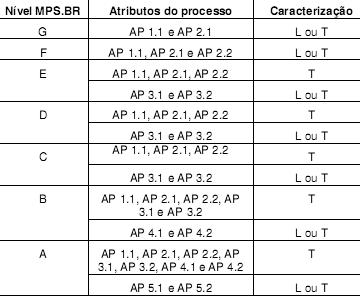
\includegraphics[width=.85\textwidth]{software-engineering/project-management/process/process-quality/mpsbr/mpsbr-ratings-uo}
	\end{block:fact}
\end{frame}


\begin{frame}
	\frametitle{MPS.BR}
	\framesubtitle{Considerações finais}
	
	\begin{block:fact}{Diferenciais}
		\begin{itemize}
			\item 7 níveis de maturidade
			\begin{itemize}
				\item implantação mais gradual
				\item maior visibilidade dos resultados de melhoria de processo
				\item prazos mais curtos
			\end{itemize}
			
			\item Compatibilidade com CMMI, conformidade com as normas ISO/IEC 15504
			e 12207.
			
			\item Adaptado para a realidade brasileira (foco em micro, pequenas e
			médias empresas).
			
			\item Custo acessível (em R\$)
		\end{itemize}
	\end{block:fact}
\end{frame}



\begin{frame}
	\frametitle{MPS.BR}
	\framesubtitle{Considerações finais}
	
	\begin{block:fact}{MPS.BR e CMMi}
		\centering
		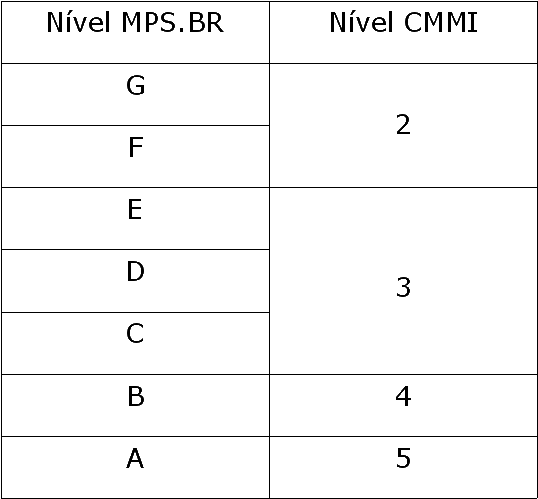
\includegraphics[width=.7\textwidth]{software-engineering/project-management/process/process-quality/mpsbr/mpsbr-cmmi}
	\end{block:fact}
\end{frame}

%\subsection{Simulação de processos}
%\begin{frame}[parent={ie:agenda}, hasnext=true, hasprev=false]
	\frametitle{Simulação de processos}

	\begin{block:concept}{Modelos de simulação}
		Abordagem para realizar a execução do modelo de processo sem utilizar 
		recursos, pessoas e ferramentas reais.
	\end{block:concept}

	
	\begin{block:fact}{Motivação}
		\begin{itemize}
			\item Analisar o comportamento de processos complexos.
			\note{
				\textbf{Sistemas dinâmicos complexos:}
				\begin{itemize}
					\item Entender a complexidade estática não é o mesmo que entender a complexidade
					dinâmica dos processos.
				
					\item Processos não são determinísticos (possuem várias opções) e muitas vezes
					são probabilísticos.
				\end{itemize}
			}
				
			\item Custo mais baixo que abordagens usuais para análise da dinâmica de processos.
			\note{
				
				\textbf{Avaliação:}
				Método usual envolve a condução de estudos experimentais (estudos de casos,
				experimentos controlados) e analisar os resultados desses estudos, o que demanda
				tempo e recursos (financeiros e humanos) consideráveis.
			}
		\end{itemize}
	\end{block:fact}
	
	\note{ 
		
		\textbf{Moral da história:}
		Desta forma, simulação de processos de software apresenta-se como um instrumento
		importante para auxiliar a tomada de decisões durante o gerenciamento de projetos de
		software.
	}
\end{frame}


\begin{frame}[hasnext=true, hasprev=true]
	\frametitle{Simulação de processos}

	\begin{block:fact}{}
		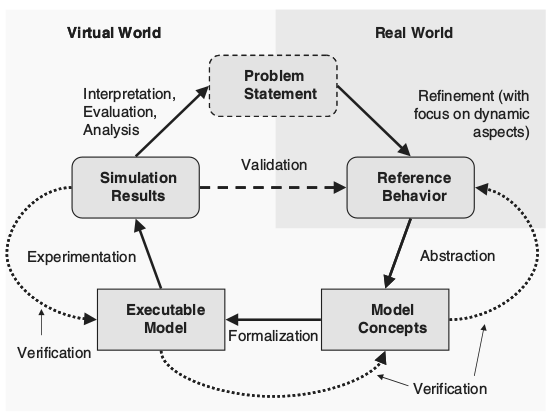
\includegraphics[width=\textwidth]{simulation-modeling-aspects}
		\cite{Muller-Pfahl:2008}
	\end{block:fact}
\end{frame}


\begin{frame}
	\frametitle{Simulação de processos}
	\framesubtitle{Formulação do problema}
	
	\begin{block:concept}{Definição}
		Estabelece o objetivo do modelo de simulação (propósito) e define o escopo
		das atividades de modelagem.
	\end{block:concept}
	
	\begin{block:concept}{Características~\cite{Kelner-etal:1999}}
		\textbf{Propósito}
		\begin{itemize}
			\item Gestão estratégica, operacional, planejamento e controle
			\item Melhoria de processo, adoção de tecnologia
			\item Compreensão do processo, treinamento
		\end{itemize}
		
		\textbf{Escopo}
		\begin{itemize}
			\item Fase do ciclo de vida em que é aplicável
			\item Projeto
			\item Diversos projetos em paralelo
			\item Linha de produto
		\end{itemize}
	\end{block:concept}
\end{frame}


\begin{frame}
	\frametitle{Simulação de processos}
	\framesubtitle{Comportamento de referência}
	
	\begin{block:concept}{Definição}
		Comportamento de referencia captura a variação (dinâmica, dependente de
		tempo) de atributos	importantes de entidades do elemento tratado pela simulação.
		\note{
			Identifica elementos de saída do modelo, permitindo a comparação com
			comportamento observável no mundo real.
		}
	\end{block:concept}
	
	\begin{block:fact}{Exemplos}
		\begin{itemize}
			\item Qualidade
			\item Esforço
			\item Custo
			
			\item Gestão operacional, planejamento e controle
			\item Melhoria de processo
			\item Adoção de tecnologia
			\item Compreensão do processo
			\item Treinamento
		\end{itemize}
	\end{block:fact}
\end{frame}


\begin{frame}
	\frametitle{Simulação de processos}
	\framesubtitle{Conceitos do modelo / Modelagem}
	
	\begin{block:concept}{Definição}
		Abstração de comportamentos observados na realidade, capturando conhecimento
		implícito ou tácito.
	\end{block:concept}
	
	\begin{block:fact}{}
		\begin{itemize}
			\item Modelos existentes de processo, qualidade e recursos.
			\item Regras de decisão (implícitas ou explícitas).
			\item Padrões de comportamento observáveis.
			\item Fluxos de informações organizacionais.
			\item Políticas
		\end{itemize}
	\end{block:fact}
\end{frame}



\begin{frame}
	\frametitle{Simulação de processos}
	\framesubtitle{Modelo de simulação}
	
	\begin{block:concept}{Definição}
		Transformação do modelo de processo em um modelo executável.
		\note{
			Deve-se buscar alinhamento entre a linguagem utilizada para definir o
			modelo de processo e a linhagem do modelo executável. Por exemplo, BPMN.
		}
	\end{block:concept}
\end{frame}


\begin{frame}
	\frametitle{Simulação de processos}
	\framesubtitle{Execução e calibração do modelo}
	
	\begin{block:concept}{Definição}
		Execução do modelo, obtendo-se resultados úteis para tratar o objetivo. Todavia,
		antes deve ocorrer a calibração dos parâmetros do modelo de simulação com
		dados reais.
	\end{block:concept}
\end{frame}


\begin{frame}
	\frametitle{Simulação de processos}
	\framesubtitle{Técnicas para simulação}
	
	\begin{block:concept}{Técnicas}
		\begin{itemize}
			\item Sistema de eventos discretos
			\note{
				Modelo baseado em evento atualiza os valores das variáveis do modelo
				conforme ocorrem eventos.
			}
			\item Sistema dinâmico
			\note{
				Modelo contínuo atualiza o valor das variáveis do modelo de acordo
				com um conjunto bem definido de equações, considerando passos precisos
				e equidistantes de tempo.
				
				Representado por equações diferenciais que, durante a simulação, são
				integradas numericamente.
			}
			\item Híbridos
		\end{itemize}
	\end{block:concept}
\end{frame}


\begin{frame}
	\frametitle{Simulação de processos}
	\framesubtitle{Exemplo:ISDMeLO}
	
	\begin{block:fact}{Simulação do ISDMeLO}
			Processo para desenvolvimento de objetos de aprendizagem segundo ADDIE, ciclo de
			vida em batelada (``cascata'').
	\end{block:fact}
	
	\begin{block:fact}{Características da simulação}
		\begin{itemize}
			\item Sistema de eventos discretos
			\item Ferramenta utilizada: Arena
		\end{itemize}
	\end{block:fact}
\end{frame}


\begin{frame}
	\frametitle{Simulação de processos}
	\framesubtitle{Limitações}
	
	\begin{block:fact}{Limitações}
		\begin{itemize}
			\item Qualidade dos resultados da simulação depende da qualidade do modelo
			e dos valores atribuídos às variáveis.
			\begin{itemize}
				\item Valores devem ser precisos e refletir o cenário real.
			\end{itemize}
			
			\item Dificuldade em definir bons modelos.
		\end{itemize}
	\end{block:fact}
\end{frame}


%\subsubsection{Próximos passos}
%\begin{frame}[parent={ie:agenda}, hasnext=true, hasprev=false]
	\frametitle{Considerações finais}

	
	\begin{block:fact}{Atualmente\ldots}
		\begin{itemize}
			\item Integração entre desenvolvimento de software e sistema~\cite{Boehm-Lane:2010}.
			
			\item Consolidação de modelos ágeis: iterativos, incrementais e centrados no usuário.
			
			\item Integração de métodos:
			\begin{itemize}
				\item Application Life-cycle Management (ALM)
				\item Continuous *
				\item DevOps (Development + Operation)
			\end{itemize}
		\end{itemize}
	\end{block:fact}
	
	\begin{block:fact}{Limitações}
		\begin{itemize}
			\item Poucos trabalhos avaliam empiricamente os diferentes tipos de
			ciclo de vida~\cite{Benediktsson-etal:2006}.
			
			\item One size does not fit all.
		\end{itemize}
	\end{block:fact}
	
	\note{
		\begin{itemize}
			\item Mais de 30 anos para adotar modelos iterativos\ldots
			
			\item Ciclos rápidos.
			
			\item DevOps (Desenvolvimento + Operacionalização)
			\begin{itemize}
				\item Continuous  planning,  collaborative  and  continuous  development,
				continuous  integration	and testing, continuous release and deployment,
				continuous infrastructure monitoring and optimization, continuous user
				behavior  monitoring  and  feedback  and  service  failure  recovery
				without  delay, etc.
			\end{itemize} 
			
			\item A integração de software e sistema é visível nos novos padrões. Por
			exemplo, colocar ambos na ISO 12207 é um recado direto de que o ciclo de
			vida do desenvolvimento de software deve considerar ambos.
		\end{itemize}
	}
\end{frame}





\backmatter{}
\part{Referências e créditos}
\part{Referências}
\section*{Referências}

\nocite{Fairley:2009}

\begin{frame}[parent={ie:agenda}, hasnext=true, hasprev=false, label=references, allowframebreaks]{\refname}
\bibliographystyle{abnt-num}
\small
\bibliography{root}
\end{frame}


\end{document}
